\documentclass[paper=a4, fontsize=11pt]{scrartcl} % KOMA-article class

%-------------------------------------------------
%   THEMES, PACKAGES, CUSTOM COMMANDS
%-------------------------------------------------
\usepackage{blindtext}
\usepackage[english]{babel}                             % English language/hyphenation
\usepackage[protrusion=true,expansion=true]{microtype}  % Better typography
\usepackage{amsmath,amsfonts,amsthm,mathtools}                    % Math packages
\usepackage[pdftex]{graphicx}                           % Enable pdflatex
\usepackage[export]{adjustbox}
\usepackage[svgnames]{xcolor}                           % Enabling colors by their 'svgnames'
\usepackage[hang, small,labelfont=bf,up,textfont=it,up]{caption} % Custom captions under/above floats
\usepackage{epstopdf}       % Converts .eps to .pdf
\usepackage{subfig}         % Subfigures
\usepackage{booktabs}       % Nicer tables
\usepackage{fix-cm}         % Custom fontsizes
\usepackage{listings}
\usepackage{soul}

\usepackage[foot=20pt,margin=1in]{geometry}

% Custom sectioning (sectsty package)
\usepackage{sectsty}
\allsectionsfont{
    \usefont{OT1}{phv}{b}{n}    % bch-b-n: CharterBT-Bold font
}
\sectionfont{
    \usefont{OT1}{phv}{b}{n}
}

% Custom colors
\definecolor{brsugrey}{rgb}{0.9, 0.9, 0.9}
\definecolor{brsublue}{rgb}{0, 0.594, 0.949}

%
\newcommand{\upperRomannumeral}[1]{\uppercase\expandafter{\romannumeral#1}}

% Creating an initial of the very first character of the content
\usepackage{lettrine}
\newcommand{\initial}[1]{%
    \lettrine[lines=3,lhang=0.3,nindent=0em]{
        \color{brsublue}
        {\textsf{#1}}}{}}

%-------------------------------------------------
%   COMMON INFO
%-------------------------------------------------
\newcommand{\hmwkTitle}{Homework}
\newcommand{\hmwkDueDate}{Lecture date: 28 September 2016}
\newcommand{\hmwkClass}{Neural Networks}
\newcommand{\hmwkClassShort}{NN WS2016}
\newcommand{\hmwkAuthorFullName}{Minh H. Nguyen}
\newcommand{\hmwkAuthorLastName}{Nguyen}
\newcommand{\hmwkAuthorEmail}{minh.nguyen@smail.inf.h-brs.de}
\newcommand{\hmwkAuthorInstitute}{BRS University of Applied Sciences}

%-------------------------------------------------
%   HEADERS & FOOTERS
%-------------------------------------------------
\usepackage{fancyhdr}
\pagestyle{fancy}
\usepackage{lastpage}
% Header (empty)
\lhead{}
\chead{}
\rhead{}
% Footer (you may change this to your own needs)
\lfoot{\footnotesize
    \texttt{\hmwkClassShort} ~
    \textbullet ~ \hmwkAuthorLastName ~
    \textbullet ~ \hmwkTitle}
\cfoot{}
\rfoot{\footnotesize page \thepage\ of \pageref{LastPage}}  % "Page 1 of 2"
\renewcommand{\headrulewidth}{0.0pt}
\renewcommand{\footrulewidth}{0.4pt}

%-------------------------------------------------
%   TITLE & AUTHOR
%-------------------------------------------------
\usepackage{titling}

\newcommand{\HorRule}{\color{brsublue}% Creating a horizontal rule
    \rule{\linewidth}{1pt}%
    \color{black}
}

% Title
\pretitle{
    \begin{flushleft}
        \HorRule
        \fontsize{25}{25} \usefont{OT1}{phv}{b}{n} \color{gray} \selectfont
}
\title{\hmwkClass \\
       \hmwkTitle}
\posttitle{
    \par
    \end{flushleft}
}

% Author
\preauthor{
    \begin{flushleft}
        \large \lineskip 0.25em
        \usefont{OT1}{phv}{b}{sl} \color{brsublue}}

\author{\hmwkAuthorFullName}

\postauthor{
        \footnotesize
        \usefont{OT1}{phv}{m}{sl} \color{Black}
        \\\hmwkAuthorInstitute
        \\\hmwkAuthorEmail
        \par
    \end{flushleft}
    \HorRule}

% Date
\date{\hmwkDueDate}

%-------------------------------------------------
%   BEGIN
%-------------------------------------------------
\begin{document}
    \maketitle
    \thispagestyle{fancy} % Enabling the custom headers/footers for the first page

    \section*{Text Summary}

    Title: \textit{Neural Networks: A Comprehensive Foundation} by Haykin Simons, chapter 1.

    \begin{itemize}
        \item Neural Network definition:
        \begin{itemize}
            \item massively \textit{parallel}, \textit{distributed} processor
            \item made up of \textit{simple processing units}
            \item can naturally \textit{store experimental knowledge} and \textit{making it available for use}
            \item resembles the brain: (1) knowledge is acquired through learning, and (2) interneurons connection strengths (synaptic weights) are used to store the acquired knowledge.
        \end{itemize}

        \item Benefits: nonlinearity, input-output mapping, adaptivity, evidential response, contextual information, fault tolerance, VLSI implementability, uniformity of analysis and design, and neurobiological analogy.
       
        \item Model of a neuron - three basic elements:
        \begin{itemize}
            \item set of synapses (connecting links) characterized by weights: ``signal $x_j$ at input of synapse $j$ connected to neuron $k$ is multiplied by weight $w_{kj}$.''
            \item adder: linear combiner which sums weighted input signals.
            \item activation function: limits amplitude of neuron output
        \end{itemize}

        \begin{center}
            \setlength{\fboxsep}{0.5pt} %
            \setlength{\fboxrule}{0.5pt}
            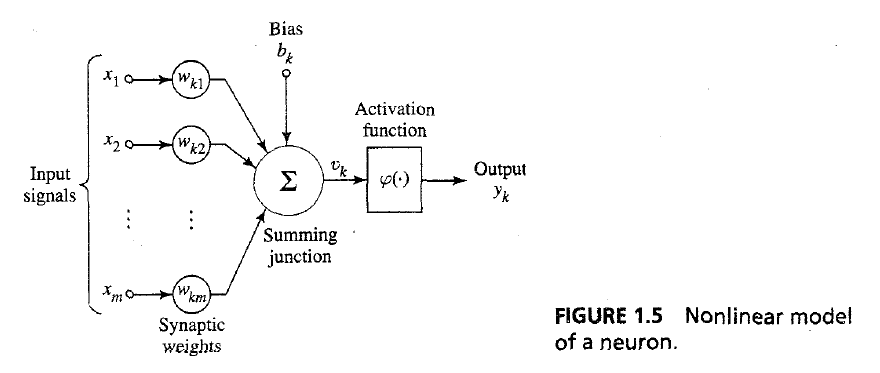
\includegraphics[width=14.0cm,fbox]{../images/Haykin-NN-figure1-5.png} %
        \end{center}

        \item Types of activation functions, $v$ being the induced local field:
        \begin{itemize}
            \item threshold function:
                \[\phi(v) =
                    \begin{dcases}
                    1, & \text{if } v \geq 0\\
                    0, & \text{if } v < 0
                    \end{dcases}
                \]
            \item Piecewise-Linear function:
                \[\phi(v) =
                \begin{dcases}
                1, & v \geq +\frac{1}{2}\\
                v, & +\frac{1}{2} > v > -\frac{1}{2}\\
                0, & v \leq -\frac{1}{2}
                \end{dcases}
                \]
            \item Sigmoid function:
                \[\phi(v) =
                \cfrac{1}{1 + exp(-av)}
                \]
                where $a$ is the slope parameter of the function.
        \end{itemize}

        \item Stochastic model of a neuron:
            \[
            x =
            \begin{dcases}
            +1 & \text{ with probability } P(v) \\
            -1 & \text{ with probability } 1 - P(v)
            \end{dcases}
            \]
            where $P(v)$ is usually
            \[
            P(v) = \cfrac{1}{1 + exp(-v/T)}
            \]
            where $T$ is a pseudotemperature which controls the uncertainty in the neuron firing.

        \item Directed graph view

        \item Feedback

        \item Network architectures:
        \begin{itemize}
            \item Single-layer Feedforward Networks
            \item Multilayer Feedforward Networks
            \item Recurrent Networks
        \end{itemize}

        \item Knowledge representation
    \end{itemize}

    \section*{Exercises}

    \subsection*{Problem 1.1}
    \[ \phi(v) = \cfrac{1}{1 + \exp(-av)} \]
    from Scipy:
    \[ \frac{d\phi}{dv} = \cfrac{a \exp(-av)}{(1 + \exp(-av))^2} \]
    \[ \Rightarrow \frac{d\phi}{dv} = a \left(\cfrac{\exp(-av)}{1 + \exp(-av)}\right) \left(\cfrac{1}{1 + \exp(-av)}\right)\]
    \[
    \Rightarrow \frac{d\phi}{dv} = a \phi(v) \left(\cfrac{1 + \exp(-av) - 1}{1 + \exp(-av)}\right)
    \Rightarrow \frac{d\phi}{dv} = a \phi(v) \left[ 1- \phi(v) \right]\]

    \[ \phi(0) = \frac{1}{2} \Rightarrow \frac{d\phi}{dv} = \frac{a}{4} \]
    $\Rightarrow$ Derivative of $\phi(v)$ is a constant around origin (scaled slope parameter).

    \subsection*{Problem 1.2}
    \[ \phi(v) = \cfrac{1 - \exp(-av)}{1 + \exp(-av)} \]
    from Scipy:
    \[ \frac{d\phi}{dv} = a \left(
                            \cfrac{(1 - \exp(-av))\exp(-av)}{(1 + \exp(-av))^2} +
                            \cfrac{\exp(-av)}{1 + \exp(-av)}
                            \right) \]
    \[ \Rightarrow \frac{d\phi}{dv} = a \left(
                            \cfrac{\exp(-av) - \exp(-2av) + \exp(-av) + \exp(-2av)}{(1 + \exp(-av))^2}
                            \right) \]
    \[ \Rightarrow \frac{d\phi}{dv} =
                        a \left(\cfrac{2\exp(-av)}{(1 + \exp(-av))^2}\right) =
                        \frac{a}{2} \left(
                        \cfrac{(1 + \exp(-av) + 1 - \exp(-av))(1 + \exp(-av) - 1 + \exp(-av))}{(1 + \exp(-av))(1 + \exp(-av))}
                        \right) 
                        \]
    \[ \Rightarrow \frac{d\phi}{dv} = \frac{a}{2}
                        \left(1 + \cfrac{1 - \exp(-av)}{1 + \exp(-av)} \right)
                        \left(1 - \cfrac{1 - \exp(-av)}{1 + \exp(-av)} \right) =
                        \frac{a}{2} (1 + \phi(v))(1 - \phi(v)) =
                        \frac{a}{2} \left[ 1 - \phi^2(v) \right]
                        \]
    \[ \phi(0) = 0 \Rightarrow \frac{d\phi}{dv} = \frac{a}{2} \]
    If $a$ is infinitely large then the $\phi(v)$ is essentially a step function at the origin.

    \newpage
    \subsection*{Problem 1.12}
    \begin{figure}[h!]
        \begin{center}
        \setlength{\fboxsep}{0.5pt} %
        \setlength{\fboxrule}{0.5pt}
        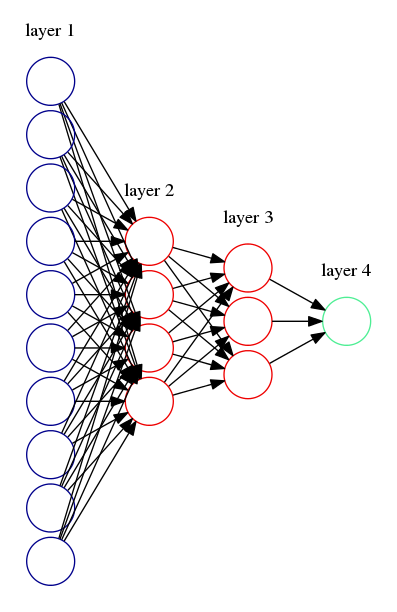
\includegraphics[width=7.0cm,fbox]{NN_MinhNguyen_20160928_ex1-12.png}
        \caption{Fully connected feedforward network with 10 source nodes, 2 hidden layers of 4 and 3 neurons, and one output neuron.}
        \end{center}
    \end{figure}

    \subsection*{Problem 1.1}

\end{document}
